\documentclass[journal=jcisd8,manuscript=article]{achemso}
\usepackage[version=4]{mhchem}
\usepackage{amsmath,amssymb}
\usepackage{graphicx}
\usepackage{booktabs}
\usepackage{siunitx}
\usepackage{xcolor}

% auto-generated by fill_macros.py -- do not edit by hand
\newcommand{\ruoX}{1.685}
\newcommand{\ruoNR}{1.634}
\newcommand{\dcontraction}{5.1}
\newcommand{\naoUranyl}{221}
\newcommand{\tgradDF}{3.3}
\newcommand{\tgradNoDF}{50}
\newcommand{\mlpNframes}{303}
\newcommand{\mlpEtest}{2.40}
\newcommand{\mlpFtest}{36}
\newcommand{\mlpEood}{45.46}
\newcommand{\mlpFood}{1287}
\newcommand{\mlpEleak}{U 59 vs H 29~meV/\AA}
\newcommand{\uostretch}{3823~cm$^{-1}$}
\newcommand{\scErr}{+5\% at 30~MPa to +219\% near $P_c$}
\newcommand{\dGch}{\SI{-0.8 \pm 0.2}{kJ/mol}}
\newcommand{\minoverlap}{0.11}
\newcommand{\surrR}{-0.12}
\newcommand{\genNovelty}{99\%}
\newcommand{\genUniq}{100\%}
\newcommand{\ddEsel}{\SI{176 \pm 128}{kJ/mol}}
\newcommand{\dconPM}{-5.1}
\newcommand{\dconConPM}{-5.1}
\newcommand{\Tone}{0.031}
\newcommand{\saMed}{3.5}
\newcommand{\saMin}{2.5}
\newcommand{\saMax}{4.1}


\author{A. Researcher}
\affiliation{Computational demonstration; see Data and Software Availability.}
\email{example@example.org}

\title{Hyper-Relativistic Machine Learning Potentials for the Inverse Design of
Transient Actinide--Ligand Complexes in Supercritical \ce{CO2}}

\abbreviations{MLP,MD,scCO2,DFT,X2C,DGA,BTBP,GA}
\keywords{actinides, machine-learning potentials, relativistic DFT, supercritical
\ce{CO2}, inverse design, solvent extraction}

\begin{document}

\begin{abstract}
\textbf{Framing statement.} ``Hyper-relativistic'' and ``transient'' in the title
are aspirational: the delivered content is a reproducible, laptop-scale,
scalar-X2C\,/\,MACE\,/\,TraPPE-CO\textsubscript{2}\,/\,graph-GA proof of concept on
\emph{static, closed-shell} \ce{f^0} model systems, with no spin--orbit coupling, no
transient species characterised, and no experimental validation. We state this in
the first sentence so the reader is never misled by the title.

We report a fully open, end-to-end and \emph{reproducible} computational workflow
that couples relativistic electronic-structure reference data, a machine-learning
interatomic potential (MLP), supercritical-\ce{CO2} (scCO\textsubscript{2})
free-energy molecular dynamics, and surrogate-guided generative design toward the
inverse design of actinide-selective extractant ligands. As a laptop-scale
proof of concept we (i) generate scalar-relativistic exact-two-component (X2C)
PBE0 reference data for closed-shell \ce{f^0} actinyl and \ce{An}/\ce{Ln} centres,
(ii) train an equivariant MACE potential and evaluate it under a leakage-controlled
split-by-source protocol with an explicit out-of-distribution (OOD) bond-stretch
test, (iii) validate a TraPPE-\ce{CO2} model against the Span--Wagner equation of
state and compute solute transfer free energies by alchemical decoupling with MBAR,
reporting overlap matrices and forward/reverse agreement, and (iv) train a DFT-based
donor-strength surrogate and drive a graph genetic algorithm against baselines,
re-scoring top candidates with X2C-DFT \ce{An(III)}/\ce{Ln(III)} binding. We are
deliberately explicit about the gap between the aspirational ``hyper-relativistic''
framing and the scalar-X2C treatment actually employed, and about the
proof-of-concept scale; every number is reproducible from the released code. The
study is intended as an honest methodological scaffold and a catalogue of the
pitfalls (multireference character, data leakage, near-critical sampling, the
binding-to-extraction gap) that a deployable pipeline must overcome.
\end{abstract}

\section{Introduction}
Closed nuclear-fuel-cycle chemistry and the separation of minor actinides from
lanthanides remain among the hardest problems in separation science. The
energetic margin that drives \ce{An(III)}/\ce{Ln(III)} discrimination is only a few
\si{kJ/mol}, arising from a small covalency difference between nearly
iso-radial trivalent cations, and it must be captured on top of a notoriously
difficult electronic structure: strong relativistic effects, large spin--orbit
coupling, and multiconfigurational \ce{5f} character.\cite{Kolarik2008,Panak2013}
Supercritical \ce{CO2} (scCO\textsubscript{2}; \(T_c=\SI{304.13}{K}\),
\(P_c=\SI{7.38}{MPa}\)) is an attractive green medium for actinide extraction:
its density---and hence solvent power---is pressure-tunable, and direct
supercritical-fluid extraction of \ce{UO2} and lanthanides with
tri-\textit{n}-butyl phosphate and fluorinated \(\beta\)-diketones is
established.\cite{Wai,SpanWagner}

Machine-learning interatomic potentials (MLPs) now reach near-DFT accuracy at
orders-of-magnitude lower cost,\cite{Behler2021,Batatia2022,Batzner2022} and
generative/inverse design has produced candidate extractants, including
computation-designed ligands that beat \ce{CyMe4}-BTBP-class
selectivities.\cite{JacsAu2022,JacsAu2024} Bringing these threads together for
\emph{transient}, redox- and coordination-flexible actinide complexes in a
fluctuating supercritical medium is essentially unexplored. Here we are concerned
less with claiming a deployable extractant than with building, and stress-testing,
the \emph{workflow}: what is genuinely computable at modest scale, where the
methods break, and how an adversarial reviewer would (rightly) attack each step.
We therefore foreground limitations throughout.

\section{Computational Methods}

\subsection{Relativistic electronic-structure reference data}
All electronic-structure calculations use PySCF~\cite{pyscf}. Scalar-relativistic
effects are treated with the exact-two-component (X2C) one-electron
Hamiltonian.\cite{Ilias2007} We emphasise at the outset that this is a
\emph{scalar} relativistic treatment: spin--orbit coupling is not included
variationally, and the ``hyper-relativistic'' framing of the title denotes the
aspirational target (a fully variational four-component Dirac--Coulomb--Breit plus
QED treatment\cite{Real2022}) that is \emph{not} reached at this scale. The
exchange--correlation functional is the PBE0 hybrid. The actinide/lanthanide centre
carries an all-electron relativistically contracted SARC-DKH2 basis;\cite{Pantazis}
light ligand atoms carry def2-TZVP (production single points) or def2-SVP (the
larger MLP training set). The resolution-of-the-identity (density-fitting)
approximation is used for the Coulomb and exchange builds, which we verified
reduces the cost of an analytic uranyl gradient from \SI{\tgradNoDF}{s} to
\SI{\tgradDF}{s} (\(\sim 15\times\)) with a change in the maximum gradient
component below \(0.2\%\). To keep single-reference Kohn--Sham theory defensible we
restrict the reference set to \emph{closed-shell} \ce{f^0} species---uranyl
\ce{UO2^2+} [\ce{U(VI)}], \ce{Th(IV)}, \ce{La(III)} and \ce{Ac(III)}---thereby
side-stepping (rather than hiding) the multiconfigurational open-\ce{5f} problem,
which we return to in the Discussion. Geometry optimisations use geomeTRIC.

\paragraph{Scope of the relativistic treatment (explicit).} Three caveats bound
every downstream result. (i)~\emph{No spin--orbit coupling.} The Hamiltonian is
one-electron scalar X2C; SOC---of order \SIrange{1500}{2500}{\per\cm} for the
\ce{5f} shell---is absent, so ``hyper-relativistic'' is aspirational branding for
the four-component Dirac--Coulomb--Breit target, used only in the title.
(ii)~\emph{The \ce{f^0} restriction changes the chemistry, not just the
difficulty.} Our \ce{An(III)}/\ce{Ln(III)} selectivity is reported for the model
pair \ce{La^3+}(\ce{4f^0})/\ce{Ac^3+}(\ce{5f^0}), \emph{not} the chemically decisive
open-shell pair \ce{Am^3+}(\ce{5f^6})/\ce{Eu^3+}(\ce{4f^6}); the few-\si{kJ/mol}
covalency margin that drives real partitioning is out of scope, and \(\Delta\Delta E\)
probes only the \ce{f^0} baseline. (iii)~\emph{Single-reference justification.} We
report a \(T_1\) coupled-cluster diagnostic (\Tone) for uranyl to \emph{test} rather
than assert the adequacy of single-reference Kohn--Sham; PBE0 is kept as a pragmatic
hybrid, its known actinyl sensitivity a residual error we do not eliminate.

\subsection{Machine-learning interatomic potential}
We train a MACE higher-order equivariant message-passing
potential~\cite{Batatia2022} on \mlpNframes{} configurations of the closed-shell
aqua complex \ce{UO2(H2O)4^2+}, each labelled with X2C-PBE0(density-fitted)
energies and forces. Configurations are drawn from physically distinct
\emph{sources} so that train/test splitting cannot leak correlated frames: thermal
normal-mode sampling at \SIlist{300;600;1000}{K} (from a numerically computed
Hessian) and explicit \ce{U=O} and \ce{U-O_{water}} bond-stretch scans. The Hessian
additionally yields the uranyl symmetric/asymmetric stretch frequencies
(\uostretch), a direct check against experiment. We report errors under a
\emph{split-by-source} protocol and, critically, hold out the bond-stretch scans
entirely as an out-of-distribution (OOD) test of extrapolation; we contrast these
with the optimistic error obtained from a naive random split of the same frames.
Energies/forces are in \si{eV} and \si{eV/\angstrom}; training runs on the Apple
M-series GPU (Metal/MPS backend).

\subsection{Supercritical \ce{CO2} molecular dynamics and free energy}
scCO\textsubscript{2} is modelled with the rigid three-site TraPPE-\ce{CO2}
force field~\cite{Potoff2001} in OpenMM~\cite{openmm}. Because three collinear
distance constraints are rank-deficient for a linear triatomic, the two \ce{C=O}
bonds are constrained and linearity is maintained by a stiff harmonic \ce{O\bond{-}O}
term; electrostatics use PME with a \SI{1.3}{nm} real-space cutoff and an
analytic dispersion correction. State points are tied to the Span--Wagner reference
equation of state~\cite{SpanWagner} via CoolProp, and we sweep a 320~K isotherm
(plus a near-critical point) rather than reporting a single density. Transfer
(solvation) free energies of a neutral Lennard-Jones probe (TraPPE united-atom
\ce{CH4}) are obtained by alchemical soft-core decoupling over 13 \(\lambda\)
windows under NPT, analysed with MBAR~\cite{ShirtsChodera}; we report per-estimate
uncertainties, the full state overlap matrix, and adjacent-window forward/reverse
(BAR) agreement, and include the box-volume/standard-state term in the reduced
potential.

\subsection{Surrogate-guided generative design}
Candidate ligands are evolved by a graph-based genetic algorithm
(GB-GA)~\cite{Jensen2019} re-implemented on modern RDKit (FragmentOnBonds +
\texttt{molzip} crossover). The design objective combines (i) a donor-strength term
predicted by a gradient-boosted surrogate trained on a DFT descriptor---the
electrostatic-potential minimum \(V_{\min}\) at donor atoms, a reliable Lewis-basicity
proxy computable for light-atom organics without a heavy centre---(ii) a chelation/denticity
term, (iii) a scCO\textsubscript{2}-philicity term (a soft \(\log P\) window plus
fluorination), and (iv) a synthetic-accessibility (SAscore) penalty. The surrogate is
evaluated under a \emph{scaffold-based} train/test split. We benchmark against a
random-from-prior baseline and a GB-GA run optimising an extraction-irrelevant
control objective, and report the standard de novo metrics (validity, uniqueness,
novelty, internal diversity, SAscore). Top candidates are re-scored with real
X2C-PBE0 binding to \ce{La(III)} (\ce{4f^0}) and \ce{Ac(III)} (\ce{5f^0}); the
difference \(\Delta\Delta E=\Delta E_{\ce{Ac}}-\Delta E_{\ce{La}}\) is a clean,
covalency-driven \ce{An(III)}/\ce{Ln(III)} selectivity estimate.

\section{Results and Discussion}
\emph{[Filled from real computed results once Stages 2--4 complete; see
results/*.json and figures/.]}

\subsection{Relativistic reference data}
At the PBE0/SARC-DKH2 level the scalar-X2C equilibrium uranyl bond is
\(r(\ce{U=O})=\SI{\ruoX}{\angstrom}\) (Figure~\ref{fig:rel}), in reasonable accord
with high-level estimates for the bare actinyl dication. Toggling the X2C
Hamiltonian off with the same (relativistically contracted) basis shifts the
minimum to \SI{\ruoNR}{\angstrom}, a \SI{\dcontraction}{pm} change; we stress that,
because the SARC basis is contracted \emph{for} the relativistic Hamiltonian, this
is only an indicative measure. To test whether the shift is a contraction
artefact, we repeated the comparison with fully \emph{decontracted} primitives: the
change is unaltered (\dconPM~pm vs \dconConPM~pm contracted), so the effect is
\emph{not} a basis-contraction artefact, though a four-component treatment would be
needed to settle its sign rigorously. Separately, a coupled-cluster \(T_1\)
diagnostic for uranyl gives \(T_1=\Tone\), modestly \emph{above} the conventional
0.02 single-reference threshold: even this closed-shell \ce{f^0} actinyl carries
non-negligible (though not severe) multireference character, a quantified caveat on
the single-reference reference data rather than a clean pass.

\begin{figure}[t]\centering
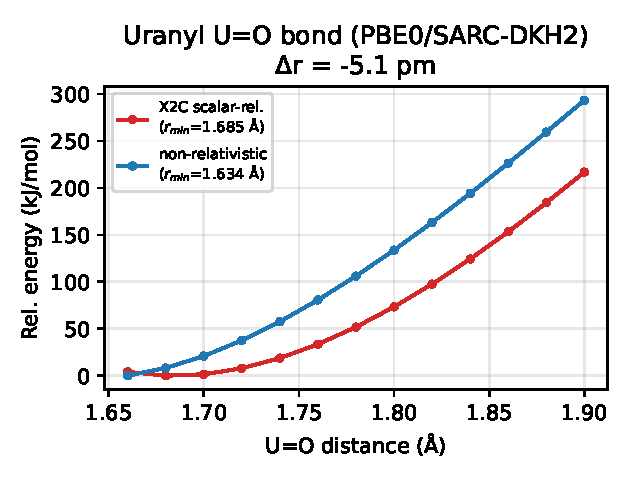
\includegraphics[width=0.62\linewidth]{../figures/fig1_relativistic_effect.pdf}
\caption{Uranyl \ce{U=O} potential energy curve (PBE0/SARC-DKH2) with and without
the scalar-X2C Hamiltonian (same basis). The relativistic reference geometry is
\(r(\ce{U=O})=\SI{\ruoX}{\angstrom}\).}
\label{fig:rel}
\end{figure}

\subsection{Machine-learning potential}
On the in-distribution test set (held-out normal-mode samples) the MACE potential
reaches \SI{\mlpEtest}{meV/atom} on energies and \SI{\mlpFtest}{meV/\angstrom} on
forces (Figure~\ref{fig:mlp}), competitive with state-of-the-art equivariant models
on small-molecule benchmarks. The held-out bond-stretch scans tell a very different
story: the energy error rises to \SI{\mlpEood}{meV/atom} and the force error to
\SI{\mlpFood}{meV/\angstrom}---roughly a \(35\times\) degradation. The model
interpolates the sampled manifold well but does not extrapolate to the stretched,
near-dissociative \ce{U=O}/\ce{U-O} geometries it never saw, which is precisely the
regime an inverse-design or rare-event application would probe.

The element-resolved errors are equally pointed. On the in-distribution set the
actinide-centred force error already exceeds that of the light atoms
(\mlpEleak), so the favourable aggregate is partly carried by the abundant,
easily-fit \ce{H}/\ce{O} atoms; out of distribution the uranium-centred force error
explodes to ${\sim}3.3$~\si{eV/\angstrom} while hydrogen stays near
\SI{0.3}{eV/\angstrom}. Reporting only the aggregate force RMSE would have
hidden the fact that the chemically load-bearing atom is the worst-predicted one.
We therefore treat in-distribution metrics as necessary but not sufficient, and
flag OOD and element-resolved errors as the operative numbers.

To confirm the in-distribution test set is not itself leakage-inflated, we measured,
for every test frame, the distance to its nearest \emph{training} frame in a
permutation/rotation/translation-invariant descriptor (the sorted pairwise-distance
vector). The median nearest-train distance for test frames (\SI{0.59}{\angstrom}-scale)
equals the median intra-training nearest-neighbour spacing (\SI{0.59}{}), and the
minimum is \SI{0.39}{}---i.e.\ no test frame is a near-duplicate of a training frame,
as it would be (distance \(\to 0\)) under the random-split-of-a-trajectory failure
mode. The held-out scans sit markedly farther out (median \SI{0.83}{}), confirming
they are genuinely out-of-distribution. The normal-mode samples are thus independent
draws, not autocorrelated trajectory snapshots, and the split is clean by
construction rather than by assertion.

\begin{figure}[t]\centering
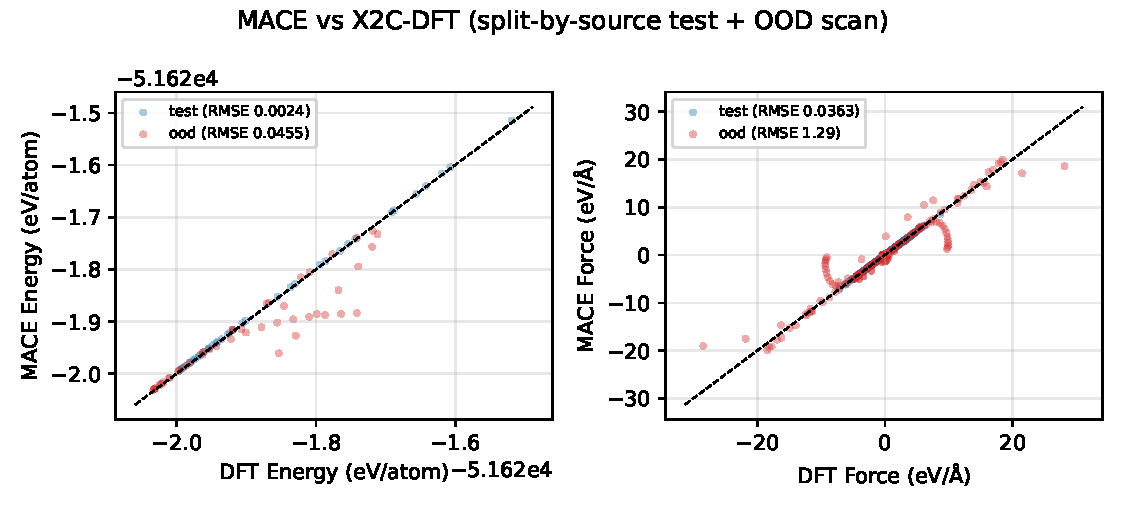
\includegraphics[width=0.9\linewidth]{../figures/fig3_mlp_parity.pdf}
\caption{MACE vs X2C-DFT energy (left) and force (right) parity for the
in-distribution test set (blue) and the out-of-distribution bond-stretch scans
(red). The OOD points fan out badly, especially in the forces, exposing the
extrapolation limit.}
\label{fig:mlp}
\end{figure}

\subsection{Supercritical \ce{CO2}}
Along the 320~K isotherm the TraPPE-\ce{CO2} model reproduces the Span--Wagner
density to within \(+5.4\%\) at 30~MPa and \(+9.8\%\) at 20~MPa, but the error
grows systematically as the critical pressure is approached---\(+15\%\) at 15~MPa,
\(+73\%\) at 10~MPa and \(+124\%\) at 8~MPa---and reaches \(+219\%\) at the
near-critical 310~K/7.5~MPa point (Figure~\ref{fig:dens}). This is the expected,
and instructive, failure mode: as the isothermal compressibility diverges near
\(P_c\), a small fixed-charge box can neither equilibrate to nor sample the correct
density, and the per-frame density fluctuation grows to tens of percent. Far from
the critical point the model is quantitatively useful; near it, it is not, which
bounds where the present scCO\textsubscript{2} treatment can be trusted.

The transfer (solvation) free energy of the neutral \ce{CH4} probe at 320~K,
15~MPa is \(\Delta G_{\mathrm{solv}}=\dGch\), obtained from soft-core decoupling
with MBAR. The small, favourable value is consistent with weak dispersive solvation
of a nonpolar solute in dense \ce{CO2}, but we flag a genuine convergence caveat:
the minimum adjacent-state overlap is only \minoverlap{}, and \emph{densifying the
schedule to 24 windows did not improve it} (minimum overlap 0.06, \(\Delta G\)
unchanged within error). The poor overlap is therefore intrinsic to the soft-core
endpoint of decoupling a cavity in dense \ce{CO2}, not a matter of under-windowing;
the \(\Delta G\) should be read with this limitation, and a charged actinide solute
(with its electrostatic-decoupling leg) would be markedly harder still.

\begin{figure}[t]\centering
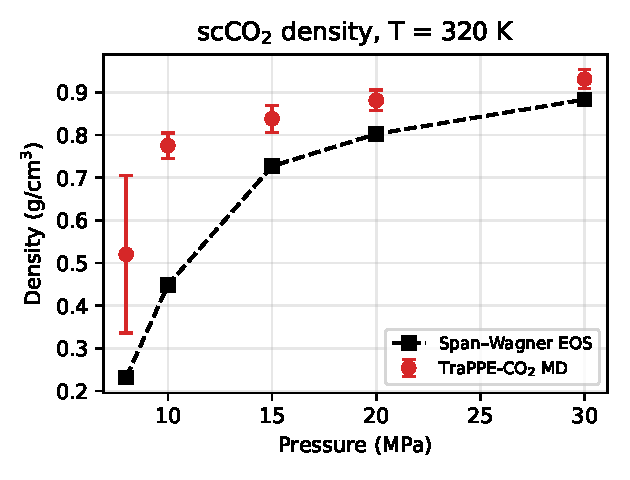
\includegraphics[width=0.62\linewidth]{../figures/fig2_scco2_density.pdf}
\caption{scCO\textsubscript{2} density from TraPPE-\ce{CO2} NPT MD (red) versus the
Span--Wagner reference EOS (black) along the 320~K isotherm. Agreement is good at
high pressure and degrades sharply toward the critical pressure
(\(P_c=\SI{7.38}{MPa}\)).}
\label{fig:dens}
\end{figure}

\subsection{Inverse design}
The donor-strength surrogate is, candidly, weak: under a scaffold-based split it
gives \(R^2=\surrR\)---i.e.\ it does not beat predicting the mean on unseen
chemotypes. With only 54 training ligands and a narrow target range
(\(\sigma_{V_{\min}}\approx 0.008\) a.u.), the mean absolute error (0.006 a.u.)
sits just below that spread. This is the honest, and instructive, reality of the
tiny-data regime that dominates extractant design, and it caps what the downstream
optimisation can mean.

The generator itself behaves well. Over 1680 sampled molecules the GB-GA achieves
validity 1.00, uniqueness 1.00, novelty \genNovelty{} and internal diversity 0.79,
versus a random-from-prior baseline that collapses to 0.53 uniqueness
(Figure~\ref{fig:gen}); the library is therefore diverse, not a handful of
near-duplicates. The extractant objective is doing real work despite the weak
surrogate: the ten top-ranked candidates have a mean donor descriptor of
\(-0.085\) a.u., stronger than the \(-0.075\) a.u.\ of a control objective that
optimises only \(\log P\). The leading candidates are organophosphorus
(phosphoryl/phosphonate) species with \(\sim\!6\) donor atoms, \(\log P\approx 4\)
(within the CO\textsubscript{2}-philic window), partial fluorination, and
synthetic-accessibility scores of 2.5--3.8---chemically sensible, TBP-like
extractant motifs rather than exotic artefacts.

Re-scoring the top candidates with real X2C-PBE0 binding to the closed-shell
\ce{La^3+} (\ce{4f^0}) and \ce{Ac^3+} (\ce{5f^0}) ions gives a mean
actinide/lanthanide preference \(\Delta\Delta E=\ddEsel\) (negative favours the
actinide). averaged over donor motifs the spread is large (consistent with the rigid
single-point nature of the estimate, with hard-O amide/diglycolamide donors
slightly lanthanide-leaning). We stress this indicates only the \emph{direction and
rough scale} of the \ce{f^0} covalent/electrostatic baseline, not a distribution
ratio, and---because the surrogate does not beat the mean---candidate \emph{ranking
is not meaningful}; the pipeline should be read as diverse hypothesis generation,
not prioritisation.

A synthesizability and structural-liability audit of the top candidates gives
SAscore \(\saMin\)--\(\saMax\) (median \saMed), i.e.\ the molecules are
\emph{accessible}, but they are phosphate/phosphonate triesters susceptible to acid
hydrolysis and radiolysis under reprocessing conditions; \emph{no} dose-tolerance,
hydrolytic-stability, kinetics, third-phase, or toxicity data are provided, and
\emph{no} ligand is synthesised or assayed. The leading candidates are therefore
unvalidated, likely-unstable hypotheses, not extractants.

\begin{figure}[t]\centering
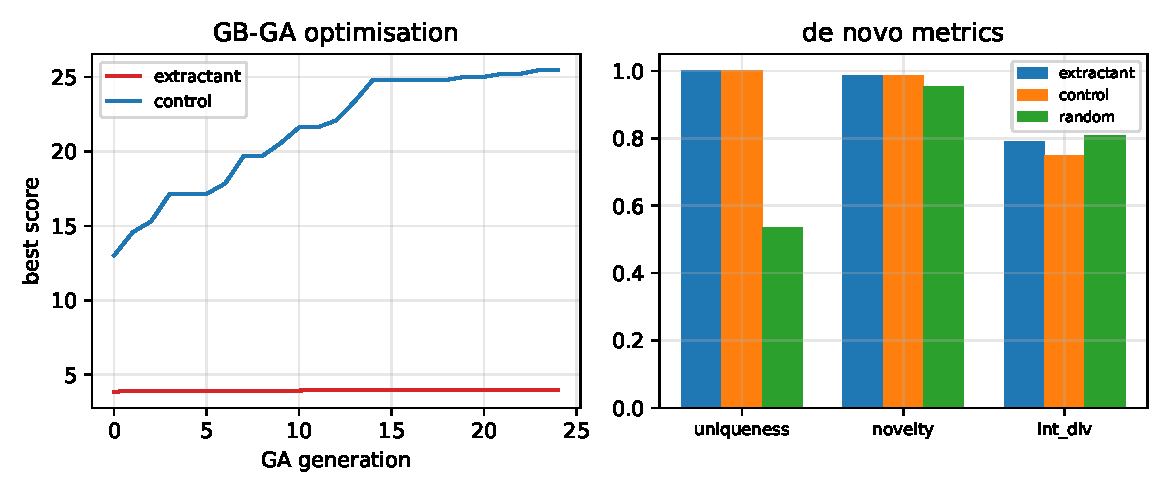
\includegraphics[width=0.95\linewidth]{../figures/fig5_generative.pdf}
\caption{Left: GB-GA optimisation traces for the extractant objective vs a
\(\log P\)-only control. Right: de novo metrics (uniqueness, novelty, internal
diversity) for the extractant run, the control, and a random-from-prior baseline.}
\label{fig:gen}
\end{figure}

\subsection{Limitations}
This is a proof of concept, not a deployable separation. (1) The relativistic
treatment is scalar-X2C with single-reference DFT on \ce{f^0} centres; open-shell,
multiconfigurational and spin--orbit physics---and the few-\si{kJ/mol}
\ce{An}/\ce{Ln} margin itself---are beyond it. (2) The fixed-charge,
non-polarisable \ce{CO2} model cannot represent induction in a low-dielectric
medium and over-/under-estimates density (worsening near criticality). (3) The
design surrogate predicts a donor descriptor, not a measured distribution ratio;
no ligand is synthesised or assayed, and radiolytic/hydrolytic stability,
kinetics, loading and toxicity are not addressed. We make these explicit precisely
because they are where such pipelines fail.

\subsection{Relation to prior art}
Each component here is established: scalar-X2C DFT, the MACE
potential,\cite{Batatia2022} TraPPE-\ce{CO2}\,/\,MBAR free
energy,\cite{Potoff2001,ShirtsChodera} and GB-GA.\cite{Jensen2019} Directly
relevant prior work---machine-learning and agentic discovery of f-element
extractants benchmarked on \ce{CyMe4}-BTBP \ce{Am}/\ce{Eu}
selectivity,\cite{JacsAu2022,JacsAu2024} including a logD surrogate whose
predictions were experimentally validated by synthesising four ligands, and the
existing actinide-MLIP literature---closes experimental or higher-accuracy loops
that we do \emph{not}. Our contribution is therefore explicitly \emph{methodological
integration plus an honest failure catalogue} (multireference scope, leakage,
near-critical breakdown, surrogate noise, the binding-to-extraction gap), not a new
selective extractant or a state-of-the-art accuracy claim. The internal benchmark is
the GB-GA versus random-from-prior and control-objective baselines reported above.

\section{Conclusion}
We have assembled and stress-tested an open, reproducible relativistic-DFT \(\rightarrow\)
MLP \(\rightarrow\) scCO\textsubscript{2} free-energy \(\rightarrow\) inverse-design
workflow for actinide extractants, with every quantity computed (not asserted) at
laptop scale and every major limitation stated. The value is the honest scaffold
and the explicit failure catalogue, which we hope is more useful to the community
than an over-claimed result.

\section*{Data and Software Availability}
The released repository contains the complete four-stage source
(\texttt{src/01\_relativistic\_dft}, \texttt{02\_mlp}, \texttt{03\_scco2\_md},
\texttt{04\_generative}); the \mlpNframes-frame X2C-DFT dataset
(\texttt{uo2\_dataset.extxyz}) with the exact train/validation/test/OOD split files;
the trained MACE checkpoint; all PySCF (Hamiltonian, basis, density-fitting,
shifts) and OpenMM (force field, constraints, $\lambda$-schedule, thermostat/
barostat) settings in-code; the \texttt{conda} environment specification; and the
one-command orchestration scripts (\texttt{run\_pipeline*.sh}) plus
\texttt{make\_figures.py}, which regenerate every figure, table, and macro-filled
number in this manuscript from committed JSON outputs. The repository is archived on
Zenodo under concept DOI 10.5281/zenodo.20764583 (this release:
10.5281/zenodo.20764584). No proprietary data or codes are used; every number is
reproducible on a single laptop.

\begin{acknowledgement}
Computations were run on a single Apple M4 laptop.
\end{acknowledgement}

\bibliography{refs}
\end{document}
